\documentclass[a4paper]{extarticle}
\usepackage[english]{babel}
\usepackage[utf8x]{inputenc}
\usepackage{amsmath}
\usepackage{dsfont}
\usepackage{graphicx}
\usepackage[colorinlistoftodos]{todonotes}
\usepackage{float}
\usepackage{subcaption}
\usepackage[pdftex,breaklinks,colorlinks,linkcolor=blue]{hyperref}
\usepackage{listings}
\usepackage{color}
\usepackage{tikz}
\usepackage{scrextend}
\changefontsizes[16pt]{14pt}
\usepackage{geometry}
\usepackage{scalerel,amssymb}
\def\mcirc{\mathbin{\scalerel*{\circ}{j}}}
\def\msquare{\mathord{\scalerel*{\Box}{gX}}}

\definecolor{dkgreen}{rgb}{0,0.6,0}
\definecolor{gray}{rgb}{0.5,0.5,0.5}
\definecolor{mauve}{rgb}{0.58,0,0.82}

\geometry{
 a4paper,
 total={170mm,257mm},
 left=35mm,
 right=35mm,
 top=30mm,
 bottom=33mm, 
}


\lstset{frame=tb,
  language=Python,
  aboveskip=3mm,
  belowskip=3mm,
  showstringspaces=false,
  columns=flexible,
  basicstyle={\small\ttfamily},
  numbers=none,
  numberstyle=\tiny\color{gray},
  keywordstyle=\color{blue},
  commentstyle=\color{dkgreen},
  stringstyle=\color{mauve},
  breaklines=true,
  breakatwhitespace=true,
  tabsize=3
}

\begin{document}

\begin{titlepage}
\newcommand{\HRule}{\rule{\linewidth}{0.5mm}} 

\center

{ \huge \bfseries Spin Plaquette Hamiltonian on a square lattice}\\[0.4cm] 

\vfill

\end{titlepage}


\tableofcontents
\newpage
\listoffigures

\newpage
\section{Hamiltonian}
We consider the spin plaquette model
\begin{eqnarray} \label{eq:1}
H = -J\sum_{\msquare} {\sigma_i^z \sigma_{j}^z \sigma_k^z \sigma_{l}^z} + h\sum_{i=1}^{N} \sigma_i^x
\end{eqnarray}
where $\sigma_i^{\{x,y,z\}}$ are the Pauli matrices on the lattice site $i$,$\msquare$ means the interaction is for a plaquette's on a square lattice, N is the total number of sites.

\subsection{2-Ladder}
Here we define the Hamiltonian on a geometry as shown below, the spins sits on the vertices and interacts as given in equation \ref{eq:1}
\vspace{5mm}

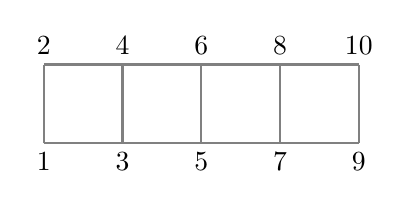
\begin{tikzpicture}
\draw  (1,0) node[anchor=north]{1} (1,1) node[anchor=south]{2} (2,0) node[anchor=north]{3} (2,1) node[anchor=south]{4} (3,0) node[anchor=north]{5} (3,1) node[anchor=south]{6} (4,0) node[anchor=north]{7} (4,1) node[anchor=south]{8} (5,0) node[anchor=north]{9} (5,1) node[anchor=south]{10} [step=1cm,gray,thick]
(1,1) grid (5,0);
\end{tikzpicture}

Now the Hamiltonian in equation \ref{eq:1} can be written as
\begin{eqnarray} \label{eq:2}
H = -J\sum_{i=1,3,5,..}^{N-3} {\sigma_i^z \sigma_{i+1}^z \sigma_{i+2}^z \sigma_{i+3}^z} + h\sum_{i=1}^{N} \sigma_i^x
\end{eqnarray}
The boundary condition used are free(open). For periodic boundary conditions the sum in the first term will go till $N-1$.


\subsubsection{Analytic Solution}

\paragraph{Domain wall variables on short rungs}


To make any further progress analytically it is useful to relable the vertices as shown in diagram below. Now we can use new domain wall variables defined on the short rungs as
\vspace{5mm}

So the Hamiltonian becomes
\begin{eqnarray} \label{eq:4}
H = -J\sum_{i=1}^{N/2} {\sigma_i^z \sigma_{i'}^z \sigma_{i+1}^z \sigma_{i'+1}^z} + h\sum_{i=1}^{N/2} (\sigma_i^x + \sigma_{i'}^x)
\end{eqnarray}

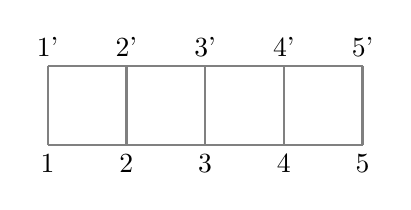
\begin{tikzpicture}
\draw  (1,0) node[anchor=north]{1} (1,1) node[anchor=south]{1'} (2,0) node[anchor=north]{2} (2,1) node[anchor=south]{2'} (3,0) node[anchor=north]{3} (3,1) node[anchor=south]{3'} (4,0) node[anchor=north]{4} (4,1) node[anchor=south]{4'} (5,0) node[anchor=north]{5} (5,1) node[anchor=south]{5'} [step=1cm,gray,thick]
(1,1) grid (5,0);
\end{tikzpicture}

\begin{eqnarray} \label{eq:5}
S_i^z = \sigma_i^z \sigma_{i'}^z \qquad S_i^x = \sigma_i^x \qquad T_i^x = \sigma_{i}^x\sigma_{i'}^x
\end{eqnarray}

Now for the $S$ variables to satisfy the pauli algebra we find $S_i^y = \sigma_i^y \sigma_{i'}^z$. Also $\sigma_{i'}^x = S_i^x T_i^x$. So the Hamiltonian in equation \ref{eq:2} can be written as

\begin{eqnarray} \label{eq:6}
H = -J\sum_{i=1}^{N/2} {S_{i}^z S_{i+1}^z} + h\sum_{i=1}^{N/2} S_i^x(1 + T_i^z)
\end{eqnarray}

Here we found that the Hamiltonian is Transverse Field Ising like in S variables but we have an extra term coupled with $S^x$ with the same coupling constant $h$. Also it is worth noticing that $T_i^x$ seperately commutes with the whole Hamiltonian. \\*


\textbf{Suggestions :} \\*

Refer garrahan's paper for 2-ladder \href{https://arxiv.org/pdf/1901.10211.pdf}{Strong zero modes in a class of generalised Ising spin ladders with plaquette interactions}.

\paragraph{Jordan Weigner transformation}


We can also think of performing a Jordan-Wiegner transformations on the original Hamiltonian(equation \ref{eq:2}) to go to the spinless fermionic variables. It is obvious to expect a plaquette interaction in the fermionic variables as well. But let's check

First we do a cannonical transformation 
\begin{eqnarray} \label{eq:7}
\sigma_z \rightarrow -\sigma_x \qquad \sigma_x \rightarrow \sigma_z
\end{eqnarray}

So the Hamiltonian in equation \ref{eq:2} becomes
\begin{eqnarray} \label{eq:8}
H = -J\sum_{i=1,3,5,..}^{N-3} {\sigma_i^x \sigma_{i+1}^x \sigma_{i+2}^x \sigma_{i+3}^x} + h\sum_{i=1}^{N} \sigma_i^z
\end{eqnarray}
Now because of the labelling used here we can introduce the transformations in the same form as for a 1D chain

\begin{eqnarray} \label{eq:9}
\sigma_i^z =  2 a_i^{\dagger} a_i - 1\\
a_i = \bigg(\prod_{j<i} \sigma_j^z \bigg) \sigma_j^+\\
a_i^{\dagger} = \bigg(\prod_{j<i} \sigma_j^z \bigg) \sigma_j^-
\end{eqnarray}

here $a_i$ and $a_i^{\dagger}$ are the anhiliation and creation operator for the fermions at site $i$. Also $\sigma^+ = \frac{1}{2} (\sigma^x + i\sigma^y)$ and $\sigma^- = \frac{1}{2} (\sigma^x - i\sigma^y)$ are raising and lowering operators at each site.
We can invert equation 9 and 10 to get $\sigma_j^+$ and $\sigma_j^-$ and then solve for $\sigma_j^x$.

\begin{eqnarray} \label{eq:10}
\sigma_i^x =  \bigg(\prod_{j<i} \sigma_j^z \bigg)(a_i + a_i^{\dagger})
\end{eqnarray}
Now we solve for the interaction term using the transformation of $\sigma_z$ and the commutation relations  $\{a_i,a_j^{\dagger}\}=\delta_{ij}$.
\begin{eqnarray} \label{eq:11}
\sigma_i^x \sigma_{i+1}^x \sigma_{i+2}^x \sigma_{i+3}^x = (a_i + a_i^{\dagger}) \sigma_i^z (a_{i+1} + a_{i+1}^{\dagger}) (a_{i+2} + a_{i+2}^{\dagger}) \sigma_{i+2}^z (a_{i+3} + a_{i+3}^{\dagger})\\
\sigma_i^x \sigma_{i+1}^x \sigma_{i+2}^x \sigma_{i+3}^x = (a_i - a_i^{\dagger}) (a_{i+1} + a_{i+1}^{\dagger}) (a_{i+2} - a_{i+2}^{\dagger}) (a_{i+3} + a_{i+3}^{\dagger})
\end{eqnarray}

Does not seem to be useful as there are quartic interaction in these variables as well. Going to Majorana fermions will not help again.

We can try to do this for the Hamiltonian in equation \ref{eq:6} which has only quadratic terms but has an extra term coupled to the $S_i^x$. Let's see how is that going to affect the form of the transformed Hamiltonian from the Ising case.



\clearpage

\subsubsection{Numerics}
We numerically diagonalize the Hamiltonian and plot the energy spectrum as shown in figure . The gap between the ground state and the lowest excited state is aslo plotted. The average magnetization $\langle m_z \rangle$ defined as 
\begin{eqnarray} \label{eq:3}
\langle m_z \rangle = \frac{1}{N} \sum_{i=1}^{N} \langle \sigma_i^z \rangle 
\end{eqnarray}
where $\langle \sigma_i^z \rangle = \langle \psi | \sigma_i^z | \psi \rangle$ is also plotted for the ground state with $h$.

%\begin{figure}[h]
%  \centering
%  \includegraphics[width=1.1\linewidth]{plots/pl_is_all_E_fbc}
%  \caption{$N=6$, $j=1$, Energy of all the levels with h, free boundary condition.}
%\end{figure}

\begin{figure}[h!]
  \begin{subfigure}[h]{0.95\textwidth}
        \includegraphics[height=.73\linewidth]{../plots/pl_is_all_E_fbc}
        \caption{free boundary condition}
        \label{fig:fbc}
    \end{subfigure}
  \begin{subfigure}[h]{0.95\textwidth}
        \includegraphics[height=.73\linewidth]{../plots/pl_is_all_E}
        \caption{periodic boundary condition}
        \label{fig:pbc}
    \end{subfigure}
    \caption[Energy of all the levels with h.]{$N=6$, $j=1$, Energy of all the levels with h.}
    \label{fig:Evsh}
\end{figure}


\begin{figure}[h!]
  \begin{subfigure}[h]{0.95\textwidth}
        \includegraphics[height=.73\linewidth]{../plots/pl_is_all_fbc}
        \caption{free boundary condition}
        \label{fig:fbc}
    \end{subfigure}
  \begin{subfigure}[h]{0.95\textwidth}
        \includegraphics[height=.73\linewidth]{../plots/pl_is_all}
        \caption{periodic boundary condition}
        \label{fig:pbc}
    \end{subfigure}
    \caption[Energy gap (with the ground state) of all the levels with h.]{$N=6$, $j=1$, Energy gap (with the ground state) of all the levels with h.}
    \label{fig:Egvsh}
\end{figure}

\begin{figure}[h!]
  \begin{subfigure}[h]{0.95\textwidth}
        \includegraphics[height=.73\linewidth]{../plots/pl_ising_fbc}
        \caption{free boundary condition}
        \label{fig:fbc}
    \end{subfigure}
  \begin{subfigure}[h]{0.95\textwidth}
        \includegraphics[height=.73\linewidth]{../plots/pl_ising}
        \caption{periodic boundary condition}
        \label{fig:pbc}
    \end{subfigure}
    \caption[Energy gap (between ground state and first excited state) with h with different system size.]{$N=6$, $j=1$, Energy gap (between ground state and first excited state) with h and different colours are different system size.}
    \label{fig:Egvsh_fes}
\end{figure}

\begin{figure}[h!]
  \begin{subfigure}[h]{0.95\textwidth}
        \includegraphics[height=.73\linewidth]{../plots/pl_mz_fbc_2}
        \caption{free boundary condition}
        \label{fig:fbc}
    \end{subfigure}
  \begin{subfigure}[h]{0.95\textwidth}
        \includegraphics[height=.73\linewidth]{../plots/pl_mz_2}
        \caption{periodic boundary condition}
        \label{fig:pbc}
    \end{subfigure}
    \caption[Average magnetization of the ground state with h.]{$N=6$, $j=1$, Average magnetization of the ground state with h.}
    \label{fig:mzvsh}
\end{figure}

\clearpage

\subsection{3-Ladder}
\subsection{p-Ladder}

\end{document}
